\chapter{Implementação}	%The main chapter title
\chaptermark{Implementação}	%Short version for page header. Comment if not needed
\label{Chapter6}

Neste capitulo será descrita como a solução foi implementada, referindo os vários microsserviços e as aplicações de deteção de linguagem. Finalmente será feita uma lista das tecnologias e ferramentas usadas para realização deste protótipo.


\section{Distribuição da aplicação}
A Tabela \ref{table:distribuicaoAplicacao} descreve a atribuição dos portos de cada um dos integrantes do sistema. 

\begin{table}[H]
\caption{Distribuição da aplicação}
\label{table:distribuicaoAplicacao}
\begin{center}
\begin{tabular}{ |p{5cm}|p{5cm}|  }
\hline
\textbf{Descrição} & \textbf{Porto} \\
\hline
SandwichService & 8091\\
\hline
IngredientService &  8090\\
\hline
ReviewService &  8095\\
\hline
StoreService &  8093\\
\hline
OrderService &  8094\\
\hline
CustomerService &  8092\\
\hline
LanguageDectetionService &  5000\\
\hline
APIGateway &  8000\\
\hline
RabbitMQ &  5672\\
\hline
MySQLContainer & 3306\\
\hline
\end{tabular} 
\end{center}
\end{table}

\section{\textit{MySQL Container}}

A Figura \ref{fig:databases} enumera as bases de dados criadas para a aplicação recorrendo ao uso do \textit{software} \textit{Podman} que faz a gestão do \textit{container} de um servidor de base de dados \textit{MySQL}. As bases de dados criadas foram as seguintes:
\begin{itemize}
    \item \textit{Ingredients}: Armazena informações acerca dos ingredientes
    \item \textit{Orders}: Armazena informações acerca das encomendas
    \item \textit{Reviews}: Armazena informações acerca das críticas
    \item \textit{Sandwiches}: Armazena informações acerca dos sanduíches
    \item \textit{Stores}: Armazena informações acerca das lojas
    \item \textit{Users}: Armazena informações acerca dos utilizadores
\end{itemize}

\begin{figure}[H]
	\centering
	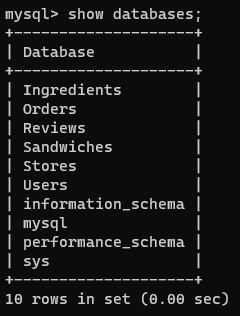
\includegraphics[scale=0.8]{databases.png}
	\caption{Bases de dados da aplicação}
	\label{fig:databases}
\end{figure}

\section{Variáveis do sistema}

As variáveis do sistema são argumentos (escritas em maiúsculas) definidos tipicamente num ficheiro à parte que podem ser acedidos pela aplicação. O uso destas variáveis é importante, dado que, podem esconder informações confidenciais, tais como, informações de acesso à base de dado e/ou informações repetitivas que podem ser reduzidas num argumento, como, por exemplo, \textit{URLs}. A Listagem \ref{lst:variavel1} apresenta os argumentos de acesso à base de dados guardados num ficheiro chamado \textit{Configuration.toml} com uma anotação no topo a referir o módulo que pode aceder aquela informação, que neste caso é o \textit{repository}.

\begin{minipage}{0.9\linewidth}
\begin{lstlisting}[language=python, caption=Definição de variáveis do sistema., label=lst:variavel1]
[ingredient.repository]
USER = "myUser"
PASSWORD = "myPassword"
HOST = "localhost"
PORT = 3306
\end{lstlisting}
\end{minipage}


Já no módulo \textit{repository}, surge o problema de como podemos aceder aos argumentos no ficheiro de configuração. Para isso é preciso recorrer à \textit{keyword configurable} que indica à aplicação que aquela variável tem que ter um valor igual ao valor do argumento com o mesmo nome no ficheiro de configuração, como pode ser visualizado na Listagem \ref{lst:variavel2}. Por isso é importante verificar-se a igualdade dos nomes para não haver variáveis que não tenham valor atribuído. 

\begin{minipage}{0.9\linewidth}
\begin{lstlisting}[language=python, caption=Invocação das variáveis do sistema., label=lst:variavel2]
configurable string USER = ?;
configurable string PASSWORD = ?; 
configurable string HOST = ?;
configurable int PORT = ?;
\end{lstlisting}
\end{minipage}

\section{Implementação dos microsserviços}
\subsection{\textit{Endpoints} do microsserviço Sanduíches}

Na Tabela \ref{table:endpoints1} são apresentados todos os \textit{endpoints} relativos ao microsserviço Sanduíche.

\begin{table}[H]
\caption{\textit{Endpoints} do microsserviço Sanduíche}
\label{table:endpoints1}
\begin{center}
\begin{tabular}{ |p{4cm}|p{6cm}|  }
\hline
\multicolumn{2}{|c|}{\textit{Endpoints}} \\
\hline
\textbf{Tipo de pedido} & \textbf{Endpoint}\\
\hline
POST & /sandwiches \\
\hline
GET & /sandwiches \\
\hline
GET & /sandwiches/searchById \\
\hline
POST & /sandwiches/descriptions \\
\hline
GET & /sandwiches/searchWithoutId \\
\hline
PUT & /sandwiches/state \\
\hline
PUT & /sandwiches/informations \\
\hline
\end{tabular} 
\end{center}
\end{table}


\subsection{\textit{Endpoints} do microsserviço Ingredientes}
Na Tabela \ref{table:endpoints2} são apresentados todos os \textit{endpoints} relativos ao microsserviço Ingredientes.

\begin{table}[H]
\caption{\textit{Endpoints} do microsserviço Ingredientes}
\label{table:endpoints2}
\begin{center}
\begin{tabular}{ |p{4cm}|p{6cm}|  }
\hline
\multicolumn{2}{|c|}{\textit{Endpoints}} \\
\hline
\textbf{Tipo de pedido} & \textbf{Endpoint}\\
\hline
POST & /ingredients \\
\hline
GET & /ingredients/searchById \\
\hline
GET & /ingredients/searchByDesignation \\
\hline
GET & /ingredients \\
\hline
PUT & /ingredients/state \\
\hline
GET & /ingredients/category \\
\hline
\end{tabular} 
\end{center}
\end{table}

\subsection{\textit{Endpoints} do microsserviço Críticas}
Na Tabela \ref{table:endpoints3} são apresentados todos os \textit{endpoints} relativos ao microsserviço Críticas.

\begin{table}[H]
\caption{\textit{Endpoints} do microsserviço Críticas}
\label{table:endpoints3}
\begin{center}
\begin{tabular}{ |p{4cm}|p{6cm}|  }
\hline
\multicolumn{2}{|c|}{\textit{Endpoints}} \\
\hline
\textbf{Tipo de pedido} & \textbf{Endpoint}\\
\hline
POST & /reviews \\
\hline
POST & /reviews/vote \\
\hline
GET & /reviews \\
\hline
GET & /reviews/reported \\
\hline
DELETE & /reviews/delete \\
\hline 
PUT & /reviews/report \\
\hline
PUT & /reviews/searchById \\
\hline
GET & /reviews/searchByClient \\
\hline
DELETE & /reviews/clientDeleteReview \\
\hline 
\end{tabular} 
\end{center}
\end{table}

\subsection{\textit{Endpoints} do microsserviço Lojas}
Na Tabela \ref{table:endpoints4} são apresentados todos os \textit{endpoints} relativos ao microsserviço Lojas.

\begin{table}[H]
\caption{\textit{Endpoints} do microsserviço Lojas}
\label{table:endpoints4}
\begin{center}
\begin{tabular}{ |p{4cm}|p{6cm}|  }
\hline
\multicolumn{2}{|c|}{\textit{Endpoints}} \\
\hline
\textbf{Tipo de pedido} & \textbf{Endpoint}\\
\hline 
POST & /stores \\
\hline
GET & /stores \\
\hline
GET & /stores/searchById \\
\hline
GET & /stores/searchByDesignation \\
\hline
GET & /stores/searchByAddress \\
\hline
DELETE & /stores/delete \\
\hline
PUT & /stores/closingHours \\
\hline
PUT & /stores/openingHours \\
\hline
\end{tabular} 
\end{center}
\end{table}

\subsection{\textit{Endpoints} do microsserviço Encomendas}
Na Tabela \ref{table:endpoints5} são apresentados todos os \textit{endpoints} relativos ao microsserviço Encomendas.

\begin{table}[H]
\caption{\textit{Endpoints} do microsserviço Encomendas}
\label{table:endpoints5}
\begin{center}
\begin{tabular}{ |p{4cm}|p{6cm}|  }
\hline
\multicolumn{2}{|c|}{\textit{Endpoints}} \\
\hline
\textbf{Tipo de pedido} & \textbf{Endpoint}\\
\hline
POST & /orders \\
\hline
GET & /orders/searchByStoreId \\
\hline
PUT & /orders/state  \\
\hline
PUT & /orders/seachByClientId \\
\hline
\end{tabular} 
\end{center}
\end{table}

\subsection{\textit{Endpoints} do microsserviço Clientes}
Na Tabela \ref{table:endpoints6} são apresentados todos os \textit{endpoints} relativos ao microsserviço Clientes.

\begin{table}[H]
\caption{\textit{Endpoints} do microsserviço Clientes}
\label{table:endpoints6}
\begin{center}
\begin{tabular}{ |p{4cm}|p{6cm}|  }
\hline
\multicolumn{2}{|c|}{\textit{Endpoints}} \\
\hline
\textbf{Tipo de pedido} & \textbf{Endpoint}\\
\hline
POST & /clients \\
\hline
GET & /clients/searchById \\
\hline
GET & /clients/searchByEmail \\
\hline
GET & /clients/searchByFiscalNumber \\
\hline
GET & /clients/authData/searchById \\
\hline
GET & /clients \\
\hline
POST & /clients/authData \\
\hline
POST & /clients/login \\
\hline
GET & /clients/data\\
\hline
\end{tabular} 
\end{center}
\end{table}

\subsection{\textit{Endpoint} do microsserviço de deteção de linguagem}
Na Tabela \ref{table:endpoints7} é apresentado o \textit{endpoint} relativos ao microsserviço de deteção de linguagem.

\begin{table}[H]
\caption{\textit{Endpoints} do microsserviço de deteção de linguagem}
\label{table:endpoints7}
\begin{center}
\begin{tabular}{ |p{4cm}|p{6cm}|  }
\hline
\multicolumn{2}{|c|}{Deteção de linguagem} \\
\hline
\textbf{Tipo de pedido} & \textbf{Endpoint}\\
\hline
POST & /language \\
\hline
\end{tabular} 
\end{center}
\end{table}

\section{API GATEWAY}

A criação de uma \textit{API GATEWAY} ajuda na implementação de segurança num certo sistema. Normalmente é utilizado em sistemas com uma arquitetura de microsserviços, no qual os vários serviços são independentes. Com este padrão de \textit{software}, os clientes podem interagir com os serviços por meio de uma interface única e unificada, dado que, os pedidos são encaminhados posteriormente para os respetivos serviços. Para além de algumas caraterísticas apresentadas anteriormente, este apresenta outras como, por exemplo:

\begin{itemize}
    \item Balanceamento de carga: Os pedidos podem ser distribuídos pelas várias instâncias
    \item Segurança: Criptógrafa o tráfego de dados e podem ser imposta políticas de segurança
    \item Limitação de taxa: Pode limitar o número de pedidos que um certo cliente pode fazer por um determinado tempo, garantindo desta forma que não haja sobrecargas ou ataques maliciosos
    \item Armazenamento em \textit{cache}: Pode armazenar em \textit{cache} respostas de serviços, levando a diminuição da latência e um aumento no desempenho
\end{itemize}

A Listagem \ref{lst:apiGateway} apresenta uma porção de código da \textit{API Gateway} desenvolvida. Para cada serviço que o sistema disponibiliza é necessária uma implementação semelhante ao código abaixo. Recorre-se a propriedade \textit{req.originalUrl} para obter-se o \textit{URL} do pedido original, por sua vez, é indispensável fazer a separação dos tipos de pedidos, dado que, no caso dos pedidos tipos \textit{GET} e \textit{DELETE}, este não precisam de um \textit{body}.

\begin{minipage}{1\linewidth}
\begin{lstlisting}[language=javascript, caption=API Gateway desenvolvida., label=lst:apiGateway]
app.all('/stores/*', (req, res) => {
    const serviceAUrl = `http://localhost:8093${req.originalUrl}`;
  
    if (req.method === 'GET' || req.method === 'DELETE') {
      axios({
        method: req.method,
        url: serviceAUrl,
        headers: req.headers
      })
        .then(response => {
          res.json(response.data);
        })
        .catch(error => {
          res.status(500).json({ error: 'An error occurred' });
        });
    } else {
      axios({
          method: req.method,
          url: serviceAUrl,
          headers: req.headers
        })
          .then(response => {
            res.json(response.data);
          })
          .catch(error => {
            res.status(500).json({ error: 'An error occurred' });
          });
    }
});
\end{lstlisting}
\end{minipage}

\section{Serviços de deteção de linguagem}

No que diz respeito a serviços de deteção de linguagem foram desenvolvidas duas aplicações recorrendo a diferentes tecnologias, como podem ser observados nas Listagens \ref{lst:python} e \ref{lst:nodejs}. Na primeira aplicação, Listagem \ref{lst:python}, foi utilizado o \textit{Python} com uma framework web denominada \textit{Flask}. Já na segunda aplicação, Listagem \ref{lst:nodejs},  foi utilizado o \textit{NodeJS} com uma framework web denominada \textit{Express.js}.

No primeiro exemplo é primariamente importado as classes \textit{Flask}, \textit{jsonify} e \textit{request} do módulo \textit{flask}, tal como, a função \textit{detect} do módulo \textit{langdetect}. Na linha a seguir é instanciado a classe \textit{Flask}. 

A seguir é definida uma rota \textit{/language} que invoca a função \textit{getLanguages()}. Quando a função for chamada a variável \textit{content} recebe os dados JSON e uma lista vazio é criada, de seguida, um \textit{loop} é utilizado, onde para cada um dos textos recebidos, é feita uma chamada à função \textit{detect}, que retorna a linguagem detetada e que é posteriormente adicionada a lista criada anteriormente para o efeito. Logo após a realização do \textit{loop} é criado um dicionário que contém as várias linguagens detetadas por ordem. Por fim, é retornado o dicionário convertido para uma resposta \textit{JSON}.

\begin{minipage}{0.9\linewidth}
\begin{lstlisting}[language=python, caption=Serviço de deteção de linguagem., label=lst:python]
from flask import Flask,jsonify,request
from langdetect import detect

app = Flask(__name__)


@app.route('/language', methods=['GET', 'POST'])
def getLanguage():
    content = request.json
    languages = []

    for text in content:
        language = detect(text["text"])
        languages.append(language)

    data = {
        "languages": languages
    }
    return jsonify(data)


if __name__ == '__main__':
    app.run()

\end{lstlisting}
\end{minipage}

Já no segundo exemplo é primariamente importado os módulos \textit{express} e \textit{languagedetect}, onde são posteriormente instanciados e no caso \textit{languagedetect} é definido o tipo de linguagem a ser apresentado. O funcionamento da obtenção das linguagens tem um esquema identifico ao referido no exemplo anterior. Sendo no final determinado o porto de funcionamento do servidor \textit{WEB}.

\begin{minipage}{0.9\linewidth}
\begin{lstlisting}[language=javascript, caption=Serviço de deteção de linguagem., label=lst:nodejs]
const express = require('express');
const app = express();
const LanguageDetect = require('languagedetect');
const lngDetector = new LanguageDetect();
lngDetector.setLanguageType("iso2");

app.use(express.json());

app.post('/language', (req, res) => {
    const content = req.body;
    let languages = [];

    content.forEach(text => {
        const language = lngDetector.detect(text.text,1);
        languages.push(language[0][0]);
    });

    data = {
        "languages":languages
    }

    res.json(data);
});

app.listen(5000, () => {
    console.log('Server running on port 5000');
});


\end{lstlisting}
\end{minipage}

Foram realizados testes com o \textit{software Postman} para verificar o funcionamento da aplicação de deteção de linguagem. Foi feito um pedido do tipo \textit{POST} ao \textit{URL http://127.0.0.1:5000/language} com uma lista de texto, um em português e outro em inglês. Ao qual foi recebido a lista das linguagens correta e na ordem correta, como se pode observar na Figura \ref{fig:testeDetecao}. Além disso, foi desenvolvido um teste de código para verificar o estado de saúde da aplicação \textit{WEB} ao longo do tempo que por sua vez que também foi bem sucedido, como se pode observar na Figura \ref{fig:testeDetecao1}.

\begin{figure}[H]
	\centering
	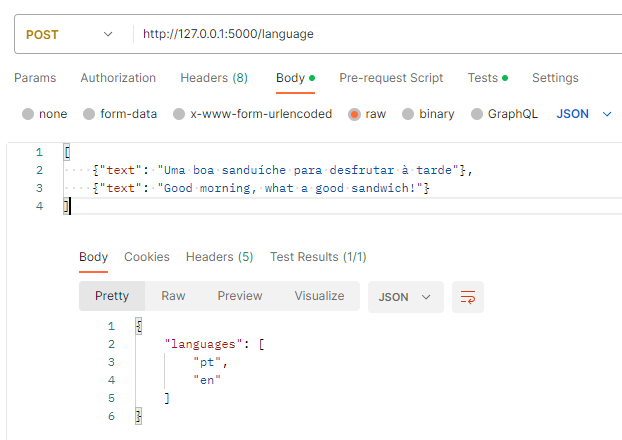
\includegraphics[scale=0.8]{testeDetecaoLinguagem.png}
	\caption{Pedido exemplo com retorno.}
	\label{fig:testeDetecao}
\end{figure}

\begin{figure}[H]
	\centering
	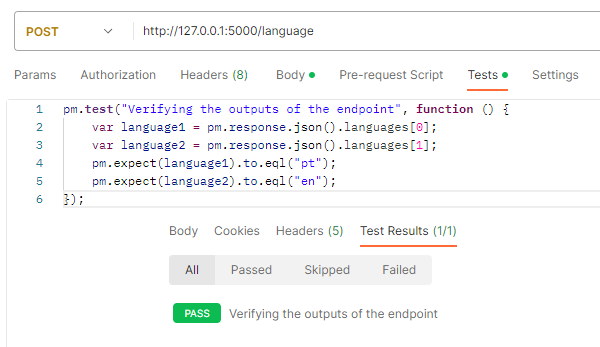
\includegraphics[scale=0.8]{testeDetecaoLinguagem1.png}
	\caption{Teste realizado ao pedido.}
	\label{fig:testeDetecao1}
\end{figure}

\section{Testes desenvolvidos}
\subsection{Teste unitário}

 apresenta um exemplo de um teste unitário desenvolvido no que diz respeito a criação de uma sanduíche. Começa-se por definir que esta porção de código é um teste com a anotação \textit{@test:Config {}}, as chavetas encontram-se vazias, dado que, não há configurações adicionais. Dado isso, é feita a invocação da função \textit{testSandwich()} que contém o código a ser executado. Essa função inicializa um o objeto \textit{SandwichDTO} com um exemplo de uma sanduíche que pode ser criada. Por fim, são feitas todas as verificações necessárias com a função \textit{assertEquals} do módulo \textit{test} para verificar se o objeto foi criado com as informações inseridas.

\begin{minipage}{1\linewidth}
\begin{lstlisting}[language=ballerina, caption=Exemplo de teste desenvolvido., label=lst:testeUnitario]
@test:Config {}
function testSandwich() {
    SandwichDTO sandwich = {designation: "Veggie Delight", selling_price: 5.99, 
        ingredients_id: [1, 2, 3], 
        descriptions: [{text: "A delicious vegetarian sandwich"}, 
                    {text: "Een heerlijk vegetarisch broodje"}]};
    test:assertEquals(sandwich.designation, "Veggie Delight");
    test:assertEquals(sandwich.selling_price, 5.99);
    test:assertEquals(sandwich.ingredients_id, [1, 2, 3]);
    test:assertEquals(sandwich.ingredients_id[0],1);
    test:assertEquals(sandwich.ingredients_id[1],2);
    test:assertEquals(sandwich.ingredients_id[2],3);
    test:assertEquals(sandwich.descriptions[0].text, "A delicious vegetarian sandwich");
    test:assertEquals(sandwich.descriptions[1].text, "Een heerlijk vegetarisch broodje");
    test:assertEquals(sandwich.descriptions.length(), 2);
    test:assertEquals(sandwich.ingredients_id.length(), 3);
}
\end{lstlisting}
\end{minipage}

\subsection{Testes de integração}

A Figura \ref{fig:testesPostman} apresenta um excerto dos testes de integração desenvolvidos para testar as funcionalidades de cada um dos serviços que fazem parte da logística do sistema. Estes forma realizados com o auxílio do \textit{software Postman}.

\begin{figure}[H]
	\centering
	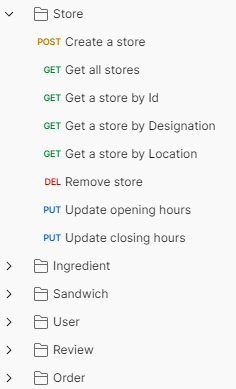
\includegraphics[scale=0.8]{figures/testesPostman.png}
	\caption{Testes desenvolvidos em Postman.}
	\label{fig:testesPostman}
\end{figure}

Já a Figura \ref{fig:testesPostman2}, nesta é demonstrado um exemplo de um \textit{script} criado, visando gerar dados que vão ser usados, neste caso, no pedido de criação de uma loja.

\begin{figure}[H]
	\centering
	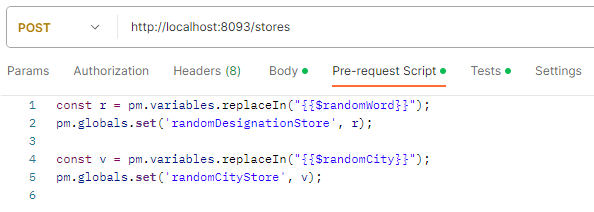
\includegraphics[scale=0.8]{figures/testesPostman2.png}
	\caption{Testes desenvolvidos em Postman.}
	\label{fig:testesPostman2}
\end{figure}

Por outro lado, a Figura \ref{fig:testesPostman1} apresenta um exemplo de testes efetuados no teste de integração. Nestes são feitos testes para verificar o código \textit{HTTP} e a presença de certos campos na resposta recebida. 

\begin{figure}[H]
	\centering
	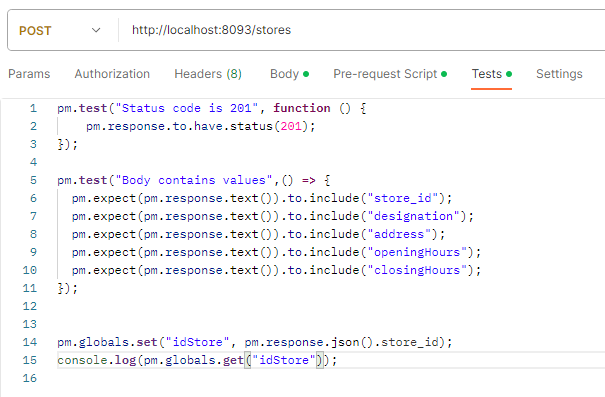
\includegraphics[scale=0.8]{figures/testesPostman1.png}
	\caption{Testes desenvolvidos em Postman.}
	\label{fig:testesPostman1}
\end{figure}

\subsection{Teste de desempenho e carga}

A Figura \ref{fig:testesCarga} apresenta testes de desempenho e carga desenvolvidos para comparar o atual desempenho do sistema com o requisito apresentado na secção Análise. Estes foram realizados com o auxílio do \textit{software JMeter}.

\begin{figure}[H]
	\centering
	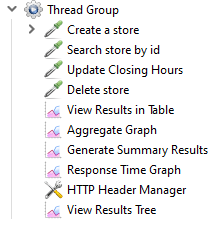
\includegraphics[scale=0.8]{figures/testesCarga.png}
	\caption{Testes de desempenho e carga.}
	\label{fig:testesCarga}
\end{figure}

Cada utilizador virtual executa o \textit{Thread Group}, este é composto por vários pedidos \textit{HTTP}, neste caso foram escolhidos um de cada tipo de pedido (\textit{POST}, \textit{GET}, \textit{PUT} e \textit{DELETE}). Este é constituído por parâmetros modificáveis, o número de utilizadores virtuais, o período de arranque e o número de vezes que o utilizador executará o mesmo. Vale a pena referir que o período de arranque representa o tempo necessário para que todos os utilizadores virtuais sejam adicionados à execução do teste.

Na Tabela \ref{table:desempenho} são apresentados vários cenários. Para cada cenário foram anotados os seguintes parâmetros:
\begin{itemize}
    \item Número de ciclos
    \item Utilizadores virtuais
    \item Taxa de transferência 
    \item Tempo decorrido
    \item Período de arranque utilizado
\end{itemize}

\begin{table}[H]
\caption{Testes de desempenho e carga}
\label{table:desempenho}
\begin{center}
\begin{tabular}{ |p{2.5cm}|p{2.5cm}|p{2.5cm}|p{2.5cm}|p{2.5cm}|  }
\hline
\multicolumn{5}{|c|}{Testes de desempenho e carga} \\
\hline
\textbf{Número de ciclos} & \textbf{Utilizadores virtuais} & \textbf{Taxa de transferência (pedidos por segundo)} & \textbf{Tempo decorrido (mm:ss.ms)} & \textbf{Período de arranque (s)}\\
\hline
1 & 10 & 232.6 & 00:00.102 & 0\\
\hline
1 & 100 & 341.0 & 00:01.230 & 1\\
\hline
1 & 1000 & 199.3 & 00:10.935 & 20\\
\hline
10 & 10 & 385.0 & 00:01.312 & 0\\
\hline
10 & 100 & 194.9 & 00:20.592 & 20\\
\hline
10 & 1000 & 332.3 & 02:00.744 & 60\\
\hline
\end{tabular} 
\end{center}
\end{table}

Para linha da tabela são apresentadas nas figuras abaixo (Figura \ref{fig:teste1}, Figura \ref{fig:teste2}, Figura \ref{fig:teste3}, Figura \ref{fig:teste4}, Figura \ref{fig:teste5} e Figura \ref{fig:teste6}) informações adicionais. Cada figura expõe a média, a mediana, o mínimo e o máximo para o número das amostras (total de pedidos realizados para cada pedido), com a adição do erro e a taxa de transferência. 

\begin{figure}[H]
	\centering
	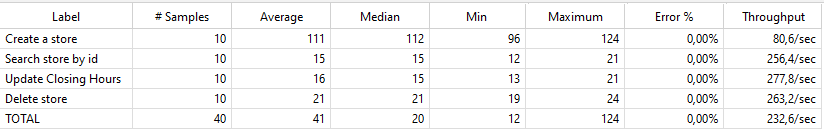
\includegraphics[scale=0.7]{figures/print1teste.png}
	\caption{Testes de desempenho e carga linha 1.}
	\label{fig:teste1}
\end{figure}
\begin{figure}[H]
	\centering
	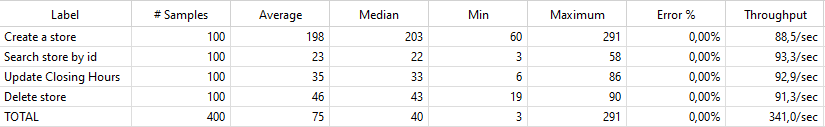
\includegraphics[scale=0.7]{figures/print2teste.png}
	\caption{Testes de desempenho e carga linha 2.}
	\label{fig:teste2}
\end{figure}

\begin{figure}[H]
	\centering
	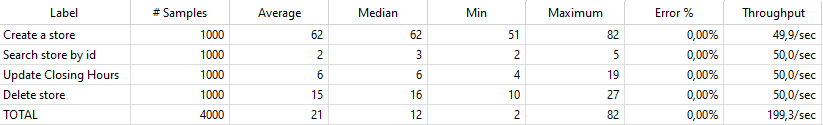
\includegraphics[scale=0.7]{figures/print3teste.png}
	\caption{Testes de desempenho e carga linha 3.}
	\label{fig:teste3}
\end{figure}

\begin{figure}[H]
	\centering
	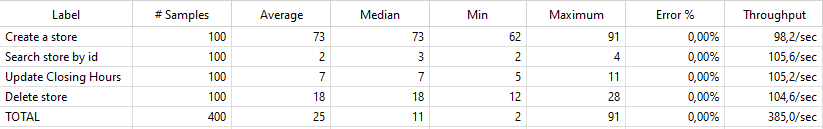
\includegraphics[scale=0.7]{figures/print4teste.png}
	\caption{Testes de desempenho e carga linha 4.}
	\label{fig:teste4}
\end{figure}

\begin{figure}[H]
	\centering
	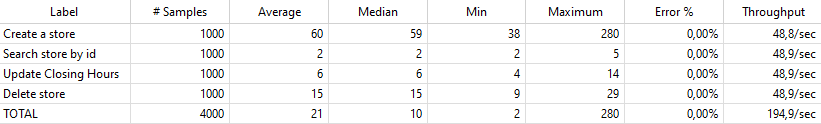
\includegraphics[scale=0.7]{figures/print5teste.png}
	\caption{Testes de desempenho e carga linha 5.}
	\label{fig:teste5}
\end{figure}

\begin{figure}[H]
	\centering
	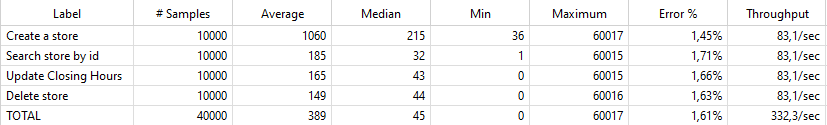
\includegraphics[scale=0.7]{figures/print6teste.png}
	\caption{Testes de desempenho e carga linha 6.}
	\label{fig:teste6}
\end{figure}

\section{Documentação da API}

Após realizada a implementação dos serviços procedeu-se a documentação dos mesmos. A Figura \ref{fig:documentacao} é um exemplo do como foi estruturada a informação para cada caso de uso. A documentação feita visa auxiliar os desenvolvedores/programadores a intenderem o funcionamento do sistema. Estes podem fornecer informações tais como:

\begin{itemize}
    \item Correspondente caso de uso
    \item O \textit{url do endpoint}
    \item Exemplo de pedido e resposta
    \item Parâmetros de consulta
    \item Possíveis respostas
\end{itemize}

\begin{figure}[H]
	\centering
	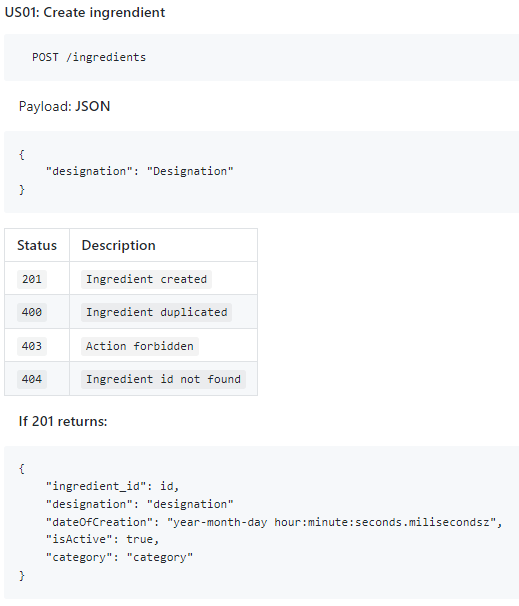
\includegraphics[scale=0.8]{figures/documentação.png}
	\caption{Documentação da API.}
	\label{fig:documentacao}
\end{figure}



\section{Tecnologias e ferramentas usadas}
Para a implementação desta solução foram usadas as seguintes tecnologias e ferramentas:

\begin{itemize}
    \item \textit{Ballerina}: Linguagem de programação
    \item \textit{MySQL}: Sistema de gestão de bases de dados
    \item \textit{Podman}: Plataforma de contentores
    \item \textit{Postman}: Ferramenta de teste para \textit{APIs}
    \item \textit{RabbitMQ}: Programa de mensagens
    \item \textit{Visual Studio Code}: Editor de código
\end{itemize}